%-------------------------------------------------------------------------
% instructions.tex
%-------------------------------------------------------------------------

%-------------------------------------------------------------------------
\setjobnamebeamerversion{fonctions-1Slide}

\usetheme{Enib}
%-------------------------------------------------------------------------

%-------------------------------------------------------------------------
\newtheorem{rem}{Remarque}[section]
\newtheorem{defin}{Définition}[section]
\newtheorem{td}{\color{blue}TD}[section]
%-------------------------------------------------------------------------

%-------------------------------------------------------------------------
\lstset
{
language=Python,
basicstyle=\ttfamily,
identifierstyle=\ttfamily,
keywordstyle=\color{blue}\ttfamily,
commentstyle=\color{gray}\ttfamily,
stringstyle=\color{green}\ttfamily,
showstringspaces=false,
extendedchars=true,
numbers=left, 
numberstyle=\tiny,
frame=lines,
linewidth=0.95\textwidth,
xleftmargin=5mm
} 
%-------------------------------------------------------------------------

%-------------------------------------------------------------------------
\def\exo#1{\mbox{}\ \hfill\mbox{\color{blue}$\rule{2mm}{2mm}\,$\footnotesize\sc TD\ref{#1}}}
\def\exercice#1#2{\mbox{}\ \ TD \ref{#1}\ #2\ \dotfill\ \pageref{#1}\mbox{}}

\newenvironment{py}[1]{\begin{minipage}[t]{#1}\footnotesize}{\end{minipage}}
%-------------------------------------------------------------------------

\graphicspath{{../../fig/}}

%-------------------------------------------------------------------------
\title[Algorithmique]{\bf Initiation à l'algorithmique}
\subtitle{\bf --- structures linéaires ---}

\author[\tt jacques.tisseau@enib.fr]{\large\bf Jacques TISSEAU}
\institute[\enib]{{\large\enib--\cerv}}
\date[enib\copyright 2009-2014]{\footnotesize enib\copyright 2009-2014}
%-------------------------------------------------------------------------

%-------------------------------------------------------------------------
\begin{document}
%-------------------------------------------------------------------------

%------------------------------------------
\begin{frame}
\frametitle{\uppercase{Informatique \hfill {S1}}}
%------------------------------------------
\titlepage

\end{frame}
\note{
\mbox{}\null\vfill

\begin{rem}[Notes de cours : couverture]
Ce support de cours accompagne le 
chapitre 4 des notes de cours « Initiation à l'algorithmique ».
$$\fbox{
\includegraphics[width=10cm,page=1]{../../../pdf/cours/info-S1.pdf}}$$
\end{rem}
}
%------------------------------------------

%------------------------------------------
\begin{frame}
\frametitle{\uppercase{Séquences}}
\framesubtitle{\uppercase{Définition}}
%------------------------------------------
\begin{description}
\item[Séquence :] suite ordonnée d'éléments,%\pause 
	éventuellement vide,%\pause
	accessibles par leur rang dans la séquence
\end{description}
%\pause
\vspace*{5mm}

Exemple de séquence : main au poker
$$
\includegraphics[width=1.25cm]{roi-pique.png}\ 
\includegraphics[width=1.25cm]{dame-pique.png}\ 
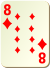
\includegraphics[width=1.25cm]{huit-carreau.png}\ 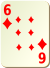
\includegraphics[width=1.25cm]{six-carreau.png}\ 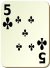
\includegraphics[width=1.25cm]{cinq-trefle.png}$$

%\pause
$$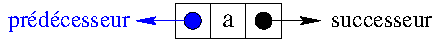
\includegraphics{sequence.pdf}$$

\end{frame}
\note{
{\bf Définitions}\begin{description}
\item[collection] regroupement fini de données 
	dont le nombre n'est pas fixé {\em a priori}.
\item[séquence] suite ordonnée d'éléments, éventuellement vide, 	accessibles par leur rang dans la séquence.
\item[arbre] collection d'éléments, appelés « n\oe uds »,
	organisés de façon hiérarchique à partir 
	d'un n\oe ud particulier, appelé la « racine » de l'arbre.
\item[graphe] collection d'éléments, appelés « sommets », et 
	de relations entre ces sommets.
\end{description}

$$\begin{tabular}{|c|c|c|}
\hline
collection & arbre & graphe \\
\hline
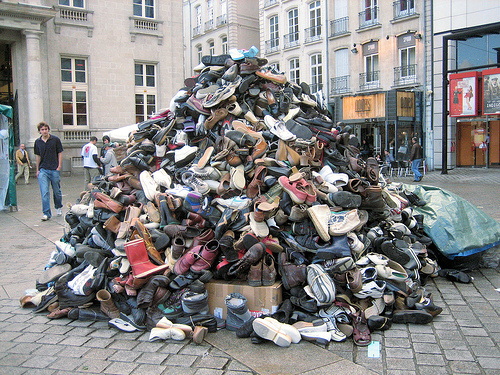
\includegraphics[width=3.5cm]{chaussures.jpg} &
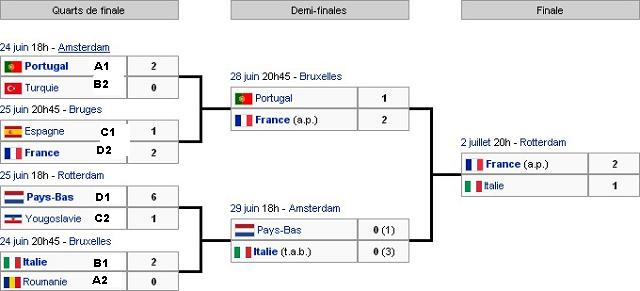
\includegraphics[width=3.5cm]{euro-2000.jpg} &
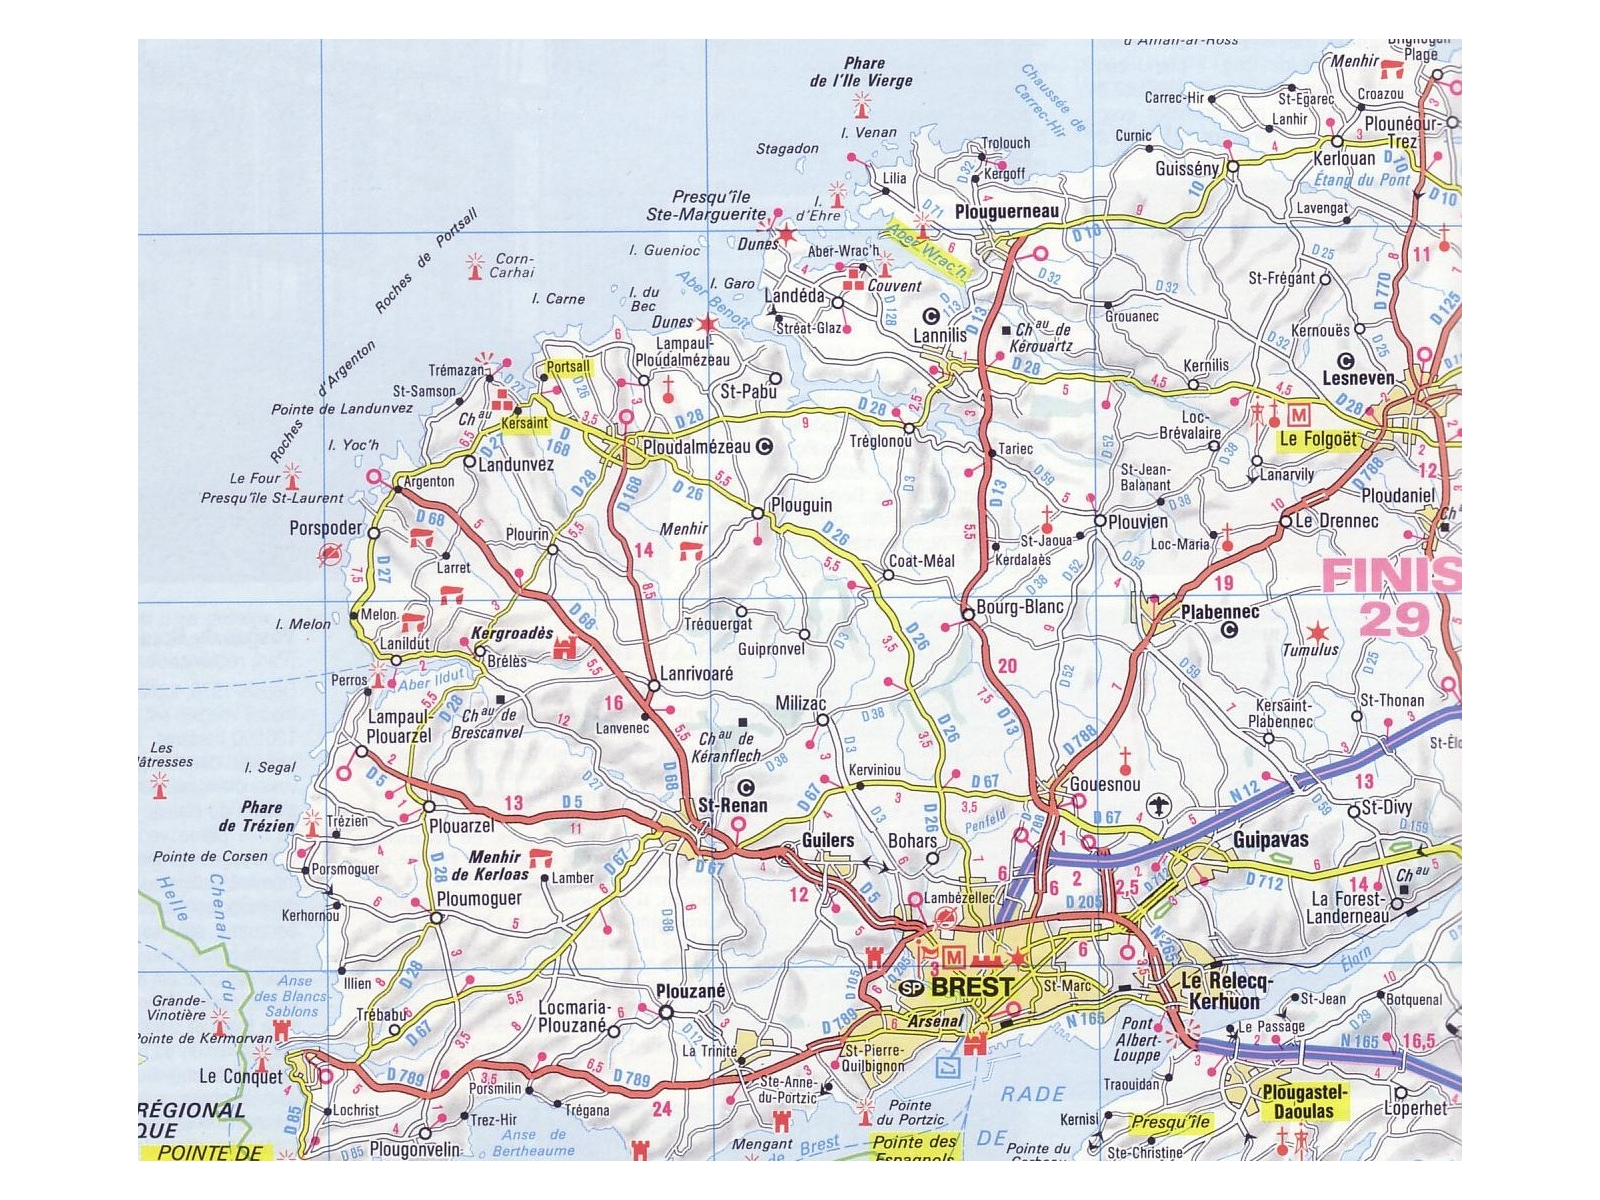
\includegraphics[width=3.5cm]{finistere-nord.jpg} \\
 &
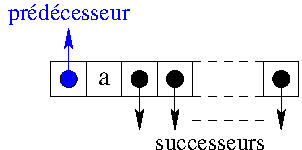
\includegraphics[width=3.5cm]{arbre.pdf} &
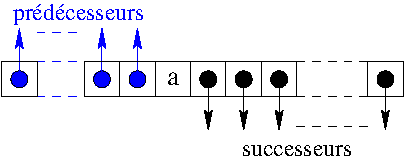
\includegraphics[width=3.5cm]{graphe.pdf} \\
\hline
\end{tabular}$$
}
%------------------------------------------


%------------------------------------------
\begin{frame}
\frametitle{\uppercase{Séquences}}
\framesubtitle{\uppercase{n-uplet, chaîne, liste}}
%------------------------------------------
\begin{columns}[T]

\column{3.5cm}
{\bf n-uplet}
%\pause

\begin{py}{3.4cm}\tt
>{>}> s = 1,7,2,4\\%\pause
>{>}> type(s)\\
<type 'tuple'>\\%\pause
>{>}> len(s)\\
4\\%\pause
>{>}> 3 in s\\
False\\%\pause
>{>}> s[1]\\
7\\%\pause
>{>}> s + (5,3)\\
(1, 7, 2, 4, 5, 3)
\end{py}
%\pause

\column{3.5cm}
{\bf chaîne}
%\pause

\begin{py}{3.4cm}\tt
>{>}> s = '1724'\\%\pause
>{>}> type(s)\\
<type 'str'>\\%\pause
>{>}> len(s)\\
4\\%\pause
>{>}> '3' in s\\
False\\%\pause
>{>}> s[1]\\
'7'\\%\pause
>{>}> s + '53'\\
'172453'
\end{py}
%\pause

\column{3.5cm}
{\bf liste}
%\pause

\begin{py}{3.4cm}\tt
>{>}> s = [1,7,2,4]\\%\pause
>{>}> type(s)\\
<type 'list'>\\%\pause
>{>}>len(s)\\
4\\%\pause
>{>}> 3 in s\\
False\\%\pause
>{>}> s[1]\\
7\\%\pause
>{>}> s + [5,3]\\
\mbox{}[1, 7, 2, 4, 5, 3]
\end{py}

\end{columns}
\end{frame}
\note{\footnotesize
$$\label{tab:sequences}\begin{tabular}{|p{4cm}|p{6cm}|}
\hline
\bf Operation on sequences & \bf Result \\
\bf ({\tt list}, {\tt tuple}, {\tt str}) &	\\
\hline
\hline
\tt x in s 		& {\tt True} if an item of {\tt s} is equal to {\tt x}, else {\tt False} \\	
\tt x not in s 		& {\tt False} if an item of {\tt s} is equal to {\tt x}, else {\tt True} \\	
\hline
\tt s1 + s2 		& the concatenation of {\tt s1} and {\tt s2} \\	 
\tt s * n, n*s 		& {\tt n} copies of {\tt s} concatenated \\	
\hline
\tt s[i] 		& {\tt i}'th item of {\tt s}, origin {\tt 0} \\	
\tt s[i:j[:step]]	& Slice of {\tt s} from {\tt i} (included) to {\tt j}(excluded). 
		  	  Optional {\tt step} value, possibly negative (default: {\tt 1}) \\ 	
\hline
\tt len(s) 		& Length of {\tt s} \\ 
\tt min(s) 		& Smallest item of {\tt s} \\
\tt max(s) 		& Largest item of {\tt s} \\
\hline
\end{tabular}$$ 
\begin{rem}[item assignment]
\begin{py}{3cm}\tt
>{>}> s = 1,7,2,4\\
>{>}> type(s)\\
<type 'tuple'>\\
>{>}> s[1] = 3\\
{\color{red}
Traceback ...\\
TypeError: 'tuple' object does not support item assignment
}\\
>{>}> s[1]\\
7
\end{py}
\hfill
\begin{py}{3cm}\tt
>{>}> s = '1724'\\
>{>}> type(s)\\
<type 'str'>\\
>{>}> s[1] = '3'\\
{\color{red}
Traceback ...\\
TypeError: 'str' object does not support item assignment
}\\
>{>}> s[1]\\
7
\end{py}
\hfill
\begin{py}{3cm}\tt
>{>}> s = [1,7,2,4]\\
>{>}> type(s)\\
<type 'list'>\\
>{>}> s[1] = 3\\
>{>}> s\\
\mbox{}[1, 3, 2, 4]\\
>{>}> s[1]\\
3
\end{py}
\end{rem}
}
%------------------------------------------


%------------------------------------------
\begin{frame}
\frametitle{\uppercase{n-uplets}}
\framesubtitle{\uppercase{séquence non modifiable d'éléments}}
%------------------------------------------
	$$\begin{tabular}{l@{ : }ll@{ : }l}
	singleton & {\tt (a)}     & paire      & {\tt (a,b)} \\%\pause
	triplet   & {\tt (a,b,c)} & quadruplet & {\tt (a,b,c,d)} \\%\pause
	\ldots    & \\
	n-uplet   & \multicolumn{3}{l}{\tt (a,b,c,d,e,f,g,h,i,j,\ldots)}
	\end{tabular}$$

%\pause
\vspace*{1cm}

\begin{columns}[T]

\column{3.25cm}
\begin{py}{3.25cm}\tt
>{>}> s = ()\\%\pause
>{>}> type(s)\\
<type 'tuple'>\\%\pause
>{>}> s = 1,7,2,4\\%\pause
>{>}> type(s)\\
<type 'tuple'>\\%\pause
>{>}> s\\
(1, 7, 2, 4)%\pause
\end{py}
\column{3.25cm}
\begin{py}{3.25cm}\tt
>{>}> s = (5)\\
>{>}> type(s)\\
<type 'int'>\\%\pause
>{>}> s = (5,)\\
>{>}> type(s)\\
<type 'tuple'>\\%\pause
>{>}> s = (5,)+()+(6,7,9)\\
>{>}> s\\
(5, 6, 7, 9)%\pause
\end{py}
\column{3.25cm}
\begin{py}{3.25cm}\tt
>{>}> s = (5,6,7,9)\\%\pause
>{>}> s[1\char`:3]\\
(6, 7)\\%\pause
>{>}> s[1\char`:]\\
(6, 7, 9)\\%\pause
>{>}> s[\char`:2]\\
(5, 6)\\%\pause
>{>}> s[-2\char`:]\\
(7, 9)
\end{py}
\end{columns}

\end{frame}
\note{
\null\vfill

\begin{td}[Division entière]
Définir une fonction qui retourne le quotient $q$ ET le reste $r$ de la 
division entière $a\div b$ ($a = bq+r$).\\
On n'utilisera pas les opérateurs prédéfinis {\tt /} et {\tt \%}.
\end{td}}
%------------------------------------------


%------------------------------------------
\begin{frame}
\frametitle{\uppercase{Chaîne de caractères}}
\framesubtitle{\uppercase{séquence non modifiable de caractères}}
%------------------------------------------

\begin{columns}[T]
\column{5.25cm}
\begin{py}{5.25cm}\tt
>{>}> s = 'une chaîne'\\%\pause
>{>}> s\\
'une chaîne'\\%\pause
>{>}> s = "une autre chaîne"\\
>{>}> s\\
'une autre chaîne'\\%\pause
>{>}> s = 'chaîne entrée sur \char`\\ \\
... plusieurs lignes'\\
>{>}> s\\
'chaîne entrée sur plusieurs lignes'\\%\pause
>{>}> s = 'chaîne entrée \char`\\n sur 1 ligne'\\
>{>}> s\\
chaîne entrée\\
\mbox{}\ sur 1 ligne
\end{py}
%\pause

\column{5.25cm}
\begin{py}{5.25cm}\tt
>{>}> s = 'c\char`\\'est ça \char`\\"peuchère\char`\\"'\\
>{>}> s\\
'c\char`\\'est ça "peuchère"'\\
>{>}> print(s)\\
c'est ça "peuchère"\\%\pause
>{>}> s = ''' a ' \char`\\\ " \char`\\n z '''\\
>{>}> s\\
' a \char`\\' \char`\\\char`\\\ " \char`\\n z '\\
>{>}> s = 'des caractères'\\
>{>}> s[9]\\
't'\\
>{>}> for c in s: print(c,end=' ')\\
... \\
d e s \  c a r a c t è r e s\\
>{>}> s[4\char`:9]\\
'carac'\\
>{>}> s[len(s)-1]\\
's'\\
>{>}> s[\char`:4] + 'mo' + s[9] + s[-1]\\
'des mots'
\end{py}
\end{columns}

\end{frame}
\note{
{\footnotesize
$$\label{tab:chaines}\begin{tabular}{|p{4cm}|p{6cm}|}
\hline
\bf Operation on {\tt str}	&	\bf Result \\
\hline
\hline
\tt s.find(sub[,start[, end]]) 			& Returns the lowest index in {\tt s} where substring {\tt sub} is found. Returns {\tt -1} if {\tt sub} is not found\\ 	
\hline
\tt s.partition(separ) 				& Searches for the separator {\tt separ} in {\tt s}, and returns a tuple {\tt (head, sep, tail)} 
			 			  containing the part before it, the separator itself, and the part after it. 
			 			  If the separator is not found, returns {\tt s} and two empty strings\\ 	
\hline
\tt s.replace(old,new[, maxCount=-1]) 			& Returns a copy of {\tt s} with the first {\tt maxCount} 
						  ({\tt -1}: unlimited) occurrences of substring {\tt old} replaced by {\tt new}\\ 	
\hline
\tt s.split([separator[, maxsplit]]) 			& Returns a list of the words in {\tt s}, using {\tt separator} as the delimiter string\\	
\hline
\end{tabular}$$
}
\null\vfill

\begin{td}[Inverser une chaîne]
\begin{enumerate}
\item Définir une fonction qui crée une copie d'une chaîne en inversant l'ordre des caractères.

\noindent\mbox{}\hspace*{1cm}\begin{py}{6cm}\tt
>{>}> inverser('inverser')\\
'resrevni'
\end{py}
\item Définir une fonction qui teste si une chaîne est un palindrome (qui se lit de la même manière de gauche à droite ou de droite à gauche : non, kayak, laval\ldots).

\noindent\mbox{}\hspace*{1cm}\begin{py}{6cm}\tt
>{>}> palindrome('kayak')\\
True
\end{py}
\end{enumerate}
\end{td}
}
%------------------------------------------


%------------------------------------------
\begin{frame}
\frametitle{\uppercase{Listes}}
\framesubtitle{\uppercase{séquence modifiable d'éléments}}
%------------------------------------------

\begin{columns}[T]
\column{5.25cm}
\begin{py}{5.25cm}\tt
>{>}> s = [1,3,5,7]\\%\pause
>{>}> s[2]\\
5\\%\pause
>{>}> s[len(s)-1]\\
7\\%\pause
>{>}> for c in s: print(c,end=' ')\\
... \\
1 3 5 7\\%\pause
>{>}> s[1\char`:3]\\
\mbox{}[3,5]\\%\pause
>{>}> s[1\char`:3] = [2,4]\\
>{>}> s\\
\mbox{}[1, 2, 4, 7]\\%\pause
>{>}> s[len(s)\char`:len(s)] = [8,9]\\
>{>}> s\\
\mbox{}[1, 2, 4, 7, 8, 9]
\end{py}
%\pause

\column{5.25cm}
\begin{py}{5.25cm}\tt
>{>}> s = [1,2,3]\\
>{>}> t = s\\
>{>}> t[0] = 9\\
>{>}> t\\
\mbox{}[9, 2, 3]\\
>{>}> s\\
\mbox{}[9, 2, 3]\\%\pause
>{>}> s = [1,2,3]\\
>{>}> t = []\\
>{>}> t[\char`:0] = s[0\char`:]\\
>{>}> t\\
\mbox{}[1, 2, 3]\\%\pause
>{>}> t[0] = 9\\
>{>}> t\\
\mbox{}[9, 2, 3]\\
>{>}> s\\
\mbox{}[1, 2, 3]
\end{py}
\end{columns}

\end{frame}
\note{\footnotesize
$$\label{tab:listes}\begin{tabular}{|p{4cm}|p{6cm}|}
\hline
\bf Operation on {\tt list}	&	\bf Result \\
\hline
\hline
\tt s[i] = x 			& item {\tt i} of {\tt s} is replaced by {\tt x} 	\\
\tt s[i:j [:step]] = t 		& slice of {\tt s} from {\tt i} to {\tt j} is replaced by {\tt t} \\	 
\tt del s[i:j[:step]] 		& same as {\tt s[i:j] = []} \\	 
\hline
\tt s.count(x) 			& returns number of {\tt i}'s for which {\tt s[i] == x} \\	 
\tt s.index(x[,start[,stop]]) 	& returns smallest {\tt i} such that {\tt s[i] == x}. 
				  {\tt start} and {\tt stop} limit search to only part 
				  of the list \\ 	
\hline
\tt s.append(x) 		& same as {\tt s[len(s) : len(s)] = [x]} \\	 
\tt s.extend(x) 		& same as {\tt s[len(s):len(s)]= x} \\	
\tt s.insert(i, x) 		& same as {\tt s[i:i] = [x] if i>= 0}. {\tt i == -1} inserts before the last element\\ 	 
\tt s.remove(x) 		& same as {\tt del s[s.index(x)]} \\
\tt s.pop([i]) 			& same as {\tt x = s[i]; del s[i]; return x} 	\\
\hline
\tt s.reverse() 		& reverses the items of {\tt s} in place \\	
\tt s.sort([cmp ]) 		& sorts the items of {\tt s} in place \\   
\hline
\end{tabular}$$ 
\null\vfill

\begin{td}[Opérations sur les listes]
Donner un exemple d'utilisation de chacune des opé\-ra\-tions  
sur les listes décrites dans le tableau ci-dessus.
\end{td}
}
%------------------------------------------


%------------------------------------------
\begin{frame}
\frametitle{\uppercase{Listes}}
\framesubtitle{\uppercase{Piles et files}}
%------------------------------------------
\begin{columns}[T]
\column{5.25cm}
{\bf Piles}
$$
\includegraphics[width=4cm]{assiettes.jpg}$$
%\pause
\begin{itemize}
\item tester si la pile est vide,
\item accéder au sommet de la pile,
\item empiler un élément au sommet de la pile,
\item dépiler l'élément qui se trouve au sommet de la pile.
\end{itemize}
%\pause

\null\vfill

\centerline{LIFO : Last In, First Out}
%\pause
\column{5.25cm}
{\bf Files}
$$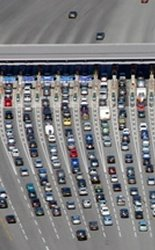
\includegraphics[height=4cm]{attente.jpg}$$
\null\vfill

\centerline{FIFO : First In, First Out}
\end{columns}

\end{frame}
\note{
\null\vfill

\begin{td}[Opérations sur les piles]
Définir les 4 opérations sur les piles : {\tt emptyStack}, {\tt topStack},
{\tt pushStack} et {\tt popStack}. 

On empilera et dépilera à la fin de la liste qui
sert à stocker les éléments de la pile.
\end{td}
\begin{td}[Opérations sur les files]
Définir les 4 opérations sur les files : {\tt emptyQueue}, {\tt topQueue},
{\tt pushQueue} et {\tt popQueue}. 

On enfilera en début de liste et on défilera à la fin de la liste qui
sert à stocker les éléments de la file.
\end{td}
}
%------------------------------------------


%------------------------------------------
\begin{frame}
\frametitle{\uppercase{Listes}}
\framesubtitle{\uppercase{Listes multidimensionnelles}}
%------------------------------------------
\begin{description}
\item[liste multidimensionnelle] liste dont les éléments sont des listes.
\end{description}
%\pause

\begin{columns}[T]
\column{5.25cm}
\begin{py}{5.25cm}\tt
>{>}> s = [[4,5],[1,2,3],[6,7,8,9]]\\%\pause
>{>}> type(s)\\
<type 'list'>\\%\pause
>{>}> len(s)\\
3\\%\pause
>{>}> type(s[2])\\
<type 'list'>\\%\pause
>{>}> s[2]\\
\mbox{}[6, 7, 8, 9]\\%\pause
>{>}> s[2][1]\\
7\\
>{>}> s[1][2]\\
3
\end{py}
%\pause

\column{5.25cm}
\begin{py}{5.25cm}\tt
>{>}> s = [[4,5],[1,2,3],[6,7,8,9]]\\
>{>}> for c in s: print(c) \\
... \\
\mbox{}[4, 5]\\
\mbox{}[1, 2, 3]\\
\mbox{}[6, 7, 8, 9]\\%\pause
>{>}> s[2]\\
\mbox{}[6, 7, 8, 9]\\%\pause
>{>}> for c in s:\\
...\ \ \ \ for e in c: print(e,end=' ')\\
...\ \ \ \ print()\\
... \\
4 5\\
1 2 3\\
6 7 8 9
\end{py}
\end{columns}

\end{frame}
\note{
\null\vfill

\begin{td}[listes multidimensionnelles]
Afficher un par un les éléments de la liste suivante :\\
{\tt s = [[[4,5],[1,2,3]], [[0],[10,11],[6,7,8,9]]]}.
\end{td}

\begin{td}[Addition de matrices]
Définir la fonction qui calcule la matrice $C$, addition
de 2 matrices $A$ et $B$ de mêmes dimensions $(n,m)$ telle que
$c_{ij} = a_{ij}\cdot b_{ij}$.
\end{td}

\begin{td}[Produit de matrices]
Définir la fonction qui calcule la matrice $C$, produit 
de 2 matrices $A$ et $B$ respectivement de dimensions $(n,r)$ et $(r,m)$.
\centerline{\mbox{}\hfill$\displaystyle c_{ij} = \sum_{k=0}^{r-1}a_{ik}\cdot b_{kj}$\hspace*{2cm} 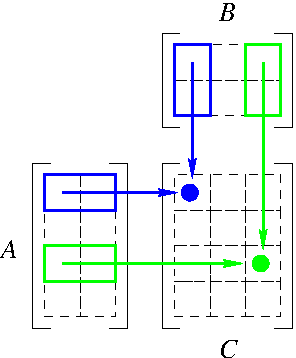
\includegraphics[height=3cm]{produit-matrices.pdf}\mbox{}\hfill}
\end{td}
}
%------------------------------------------


%------------------------------------------
\begin{frame}
\frametitle{\mbox{\uppercase{Recherche d'un élément}}}
\framesubtitle{\uppercase{Recherche séquentielle}}
%------------------------------------------
\begin{description}
\item[recherche] retrouver une information stockée en mémoire vive, sur un disque dur ou sur le réseau.
\end{description}
\centerline{\alert{Recherche dans une séquence}}
\begin{columns}[T]
\column{5.25cm}
%$$\multiinclude[graphics={width=5.5cm},format=pdf]{rechSeq}$$
$$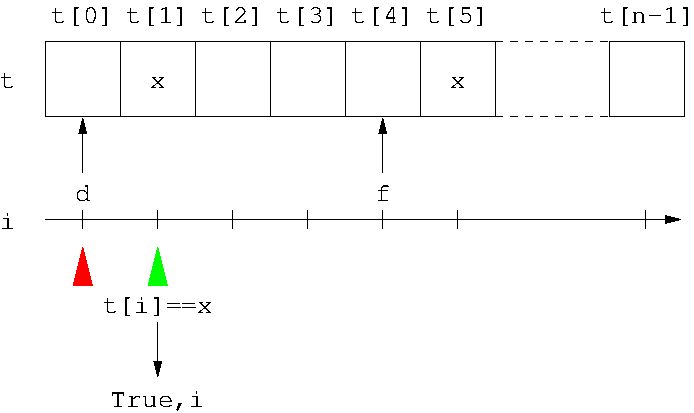
\includegraphics[width=5.5cm]{rechSeq-3}$$
%\pause
\column{5.25cm}
%$$\multiinclude[graphics={width=5.5cm},format=pdf]{rechSeqFalse}$$
$$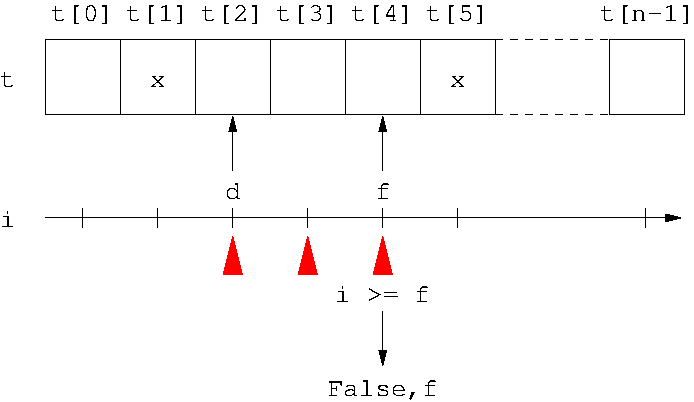
\includegraphics[width=5.5cm]{rechSeqFalse-4}$$
\end{columns}
%\pause
\vspace*{5mm}

\centerline{\alert{Complexité linéaire : $O(n)$}}
\end{frame}
\note{
\null\vfill

\begin{td}[Recherche séquentielle]
Définir une fonction de recherche séquentielle de la première occurence d'un élément 
{\tt x} dans une liste {\tt t} entre les rangs {\tt debut} (inclus) et {\tt fin} (exclu).\\
On retournera un couple de valeurs {\tt (ok,r)} : {\tt ok} est un booléen qui teste si la
recherche est fructueuse ou non et {\tt r} est le rang de la première occurence de l'élément
recherché s'il a effectivement été trouvé.

\begin{py}{7cm}\tt
>{>}> s = [1,3,5,6,5,2]\\
>{>}> recherche(s,5,0,len(s)-1)\\
(True, 2)\\
>{>}> recherche(s,5,3,len(s)-1)\\
(True, 4)\\
>{>}> recherche(s,4,0,len(s)-1)\\
(False, 6)
\end{py}
\end{td}
\begin{td}[Annuaire téléphonique]
On considère un annuaire téléphonique stocké sous la forme d'une liste de couples
{\tt (nom,téléphone)}.\\ Exemple : {\tt [('jean','0607080910'),('paul','0298000102')]}
\begin{enumerate}
\item Définir une fonction qui retrouve dans un annuaire téléphonique
	le numéro de téléphone à partir du nom.
\item Définir la fonction inverse qui retrouve 
	le nom à partir du numéro de téléphone.
\end{enumerate}
\end{td}
}
%------------------------------------------


%------------------------------------------
\begin{frame}
\frametitle{\mbox{\uppercase{Recherche d'un élément}}}
\framesubtitle{\uppercase{Recherche dichotomique}}
%------------------------------------------
\centerline{\alert{Recherche dans une séquence triée}}
%\pause
\centerline{{\tt m = (d+f)/2} : milieu de la plage de recherche}
%$$\multiinclude[graphics={width=5.5cm},format=pdf]{rechDicho}$$
$$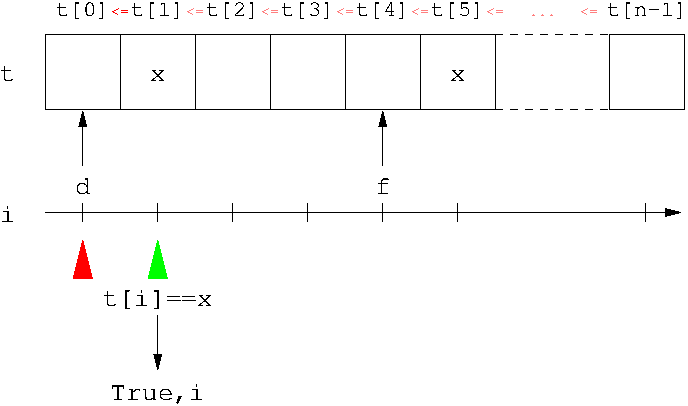
\includegraphics[width=5.5cm]{rechDicho}$$
%\pause
\begin{itemize}
\item si {\tt x == t[m]}, on a trouvé une solution et la recherche s'arrête;
%\pause
\item si {\tt x < t[m]}, poursuivre la recherche dans la moitié gauche de la liste;
%\pause
\item si {\tt x > t[m]}, poursuivre la recherche dans la moitié droite de la liste.
\end{itemize}
%\pause
\centerline{\alert{Complexité logarithmique : $O(\log(n))$}}

\end{frame}
\note{
\null\vfill

\begin{td}[Recherche dichotomique]
\begin{enumerate}
\item Définir une fonction de recherche dichotomique d'un élément 
{\tt x} dans une liste triée {\tt t} entre les rangs {\tt debut} (inclus) et {\tt fin} (exclu).\\
On retournera un couple de valeurs {\tt (ok,r)} : {\tt ok} est un booléen qui teste si la
recherche est fructueuse ou non et {\tt r} est le rang de la première occurence de l'élément
recherché s'il a effectivement été trouvé.

\begin{py}{7cm}\tt
>{>}> s = [1,3,5,6,6,9]\\
>{>}> dichotomie(s,6,0,len(s)-1)\\
(True, 4)\\
>{>}> dichotomie(s,6,2,len(s)-1)\\
(True, 3)\\
>{>}> dichotomie(s,4,0,len(s)-1)\\
(False, 1)
\end{py}
\item A priori, la recherche dichotomique obtenue n'assure pas de trouver la première occurence
d'un élément {\tt x} dans une liste {\tt t} triée.\\
Modifier l'algorithme de recherche dichotomique proposé pour rechercher la
première occurence d'un élément {\tt x} dans une liste {\tt t} triée.
\end{enumerate}
\end{td}
}
%------------------------------------------


%------------------------------------------
\begin{frame}
\frametitle{\uppercase{Tri d'une séquence}}
\framesubtitle{\uppercase{Tri par sélection}}
%------------------------------------------
\begin{description}
\item[relation d'ordre total] (notée $\leq$)
\begin{enumerate}
\item réflexivité : $x \leq x$
\item antisymétrie : $(x \leq y) \mbox{\tt\ and\ } (y \leq x) \Rightarrow x = y$
\item transitivit\'e : $(x \leq y) \mbox{\tt\ and\ } (y \leq z) \Rightarrow (x \leq z)$
\end{enumerate}
\end{description}
%\pause


$$\begin{minipage}{3.5cm}
$\begin{array}{|cccccc|}
\hline
6 & 4 & 1 & 3 & 5 & 2 \\
\hline
\end{array}$
%\pause
\vspace*{1mm}

$\begin{array}{|cccccc|}
\hline
\color{blue}\bf 1 & 4 & \color{blue}\bf 6 & 3 & 5 & 2 \\
\hline
\end{array}$
%\pause
\vspace*{1mm}

$\begin{array}{|cccccc|}
\hline
1 & \color{blue}\bf 2 & 6 & 3 & 5 & \color{blue}\bf 4 \\
\hline
\end{array}$
%\pause
\vspace*{1mm}

$\begin{array}{|cccccc|}
\hline
1 & 2 & \color{blue}\bf 3 & \color{blue}\bf 6 & 5 & 4 \\
\hline
\end{array}$
%\pause
\vspace*{1mm}

$\begin{array}{|cccccc|}
\hline
1 & 2 & 3 & \color{blue}\bf 4 & 5 & \color{blue}\bf 6 \\
\hline
\end{array}$
%\pause
\vspace*{1mm}

$\begin{array}{|cccccc|}
\hline
1 & 2 & 3 & 4 & \color{blue}\bf 5 & 6 \\
\hline
\end{array}$
%\pause
\vspace*{1mm}

$\begin{array}{|cccccc|}
\hline
1 & 2 & 3 & 4 & 5 & \color{blue}\bf 6 \\
\hline
\end{array}$
\end{minipage}$$
%\pause
\centerline{\alert{Complexité quadratique : $O(n^2)$}}
\end{frame}
\note{
\null\vfill

\begin{td}[Liste ordonnée]
Définir une fonction qui teste si une liste est triée ou non
entre les rangs {\tt debut} (inclus) et {\tt fin} (exclu).

\begin{py}{5cm}\tt
>{>}> s = [3,1,2,3,1]\\
>{>}> enOrdre(s,0,len(s)-1)\\
False\\
\end{py}
\hfill
\begin{py}{5cm}\tt
>{>}> enOrdre(s,1,3)\\
True\\
>{>}> enOrdre(s,1,4)\\
False
\end{py}
\end{td}
\begin{td}[Tri par sélection]
Définir une fonction qui trie une liste {\tt t} par la méthode du tri par sélection
entre les rangs {\tt debut} (inclus) et {\tt fin} (exclu).

\begin{py}{7cm}\tt
>{>}> s = [5,4,3,2,1,0]\\
>{>}> triSelection(s,0,len(s)-1)\\
>{>}> s\\
\mbox{}[0, 1, 2, 3, 4, 5]
\end{py}
\end{td}
\begin{td}[Tri d'un annuaire téléphonique]
On considère un annuaire téléphonique stocké sous la forme d'une liste de couples
{\tt (nom,téléphone)}. \\
Exemple : {\tt [('paul','0607080910'),('jean','0298000102')]}

Définir une fonction qui trie un annuaire téléphonique par ordre alphabétique des noms.
\end{td}
}
%------------------------------------------


%------------------------------------------
\begin{frame}
\frametitle{\uppercase{Tri d'une séquence}}
\framesubtitle{\uppercase{Tri par insertion}}
%------------------------------------------
\begin{description}
\item[tri par insertion :] trier successivement les premiers éléments de la liste
%\pause

	A la $i^{\grave eme}$ étape, on insère le $i^{\grave eme}$ élément 
	à son rang parmi les $i-1$ éléments précédents qui sont déjà triés entre eux.
\end{description}
%\pause

$$\begin{minipage}{3.5cm}
$\begin{array}{|cccccc|}
\hline
6 & \multicolumn{1}{|c}{4} & 1 & 3 & 5 & 2 \\
\hline
\end{array}$
%\pause
\vspace*{1mm}

$\begin{array}{|cccccc|}
\hline
\color{blue}\bf 4 & 6 & \multicolumn{1}{|c}{1} & 3 & 5 & 2 \\
\hline
\end{array}$
%\pause
\vspace*{1mm}

$\begin{array}{|cccccc|}
\hline
\color{blue}\bf 1 & 4 & 6 & \multicolumn{1}{|c}{3} & 5 & 2 \\
\hline
\end{array}$
%\pause
\vspace*{1mm}

$\begin{array}{|cccccc|}
\hline
1 & \color{blue}\bf 3 & 4 & 6 & \multicolumn{1}{|c}{5} & 2 \\
\hline
\end{array}$
%\pause
\vspace*{1mm}

$\begin{array}{|cccccc|}
\hline
1 & 3 & 4 & \color{blue}\bf 5 & 6 & \multicolumn{1}{|c|}{2} \\
\hline
\end{array}$
%\pause
\vspace*{1mm}

$\begin{array}{|cccccc|}
\hline
1 & \color{blue}\bf 2 & 3 & 4 & 5 & 6 \\
\hline
\end{array}$
%\pause
\end{minipage}$$
\vspace*{5mm}

\centerline{\alert{Complexité quadratique : $O(n^2)$}}
\end{frame}
\note{
\null\vfill

\begin{td}[Tri par insertion]
Définir une fonction qui trie une liste {\tt t} par la méthode du tri par insertion
entre les rangs {\tt debut} (inclus) et {\tt fin} (exclu).

\begin{py}{7cm}\tt
>{>}> s = [9,8,7,6,5,4]\\
>{>}> triInsertion(s,0,len(s)-1)\\
>{>}> s\\
\mbox{}[4, 5, 6, 7, 8, 9]\\
>{>}> s = [9,8,7,6,5,4]\\
>{>}> triInsertion(s,1,4)\\
>{>}> s\\
\mbox{}[9, 5, 6, 7, 8, 4]
\end{py}
\end{td}
}
%------------------------------------------


%------------------------------------------
\begin{frame}
\frametitle{\uppercase{Tri d'une séquence}}
\framesubtitle{\uppercase{Tri rapide}}
%------------------------------------------
\begin{columns}
\column{5.25cm}
%$$\multiinclude[graphics={width=5.5cm},format=pdf]{triRapide}$$
$$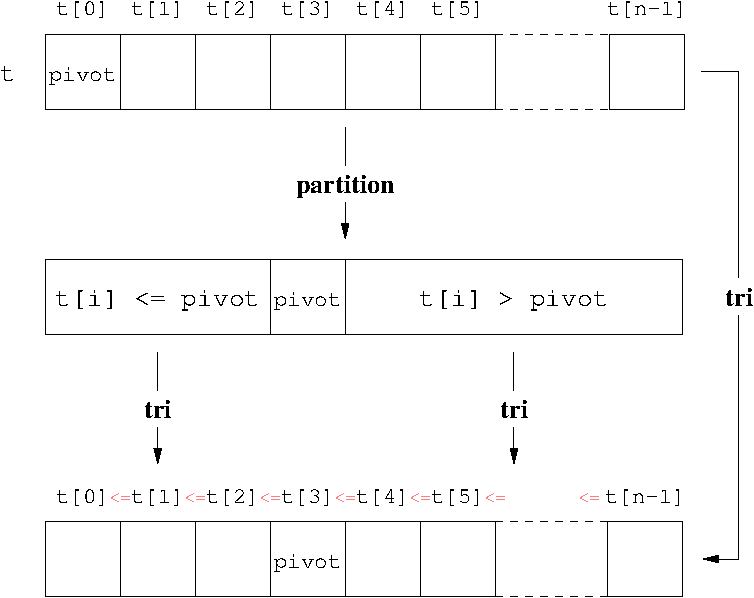
\includegraphics[width=5.5cm]{triRapide-4}$$
%\pause
\column{5.25cm}
$$\begin{minipage}{3.5cm}
$\begin{array}{|cccccc|}
\hline
6 & 4 & 1 & 3 & 5 & 2 \\
\hline
\end{array}$
%\pause
\vspace*{1mm}

$\begin{array}{|ccccc|c}
\cline{1-5}
2 & 4 & 1 & 3 & 5 & \color{blue}\bf 6\\
\cline{1-5}
\end{array}$
%\pause
\vspace*{1mm}

$\begin{array}{|c|c|ccc|c}
\cline{1-1}\cline{3-5}
1 & \color{blue}\bf 2 & 4 & 3 & 5 & 6\\
\cline{1-1}\cline{3-5}
\end{array}$
%\pause
\vspace*{1mm}

$\begin{array}{cc|c|c|c|c}
\cline{3-3}\cline{5-5}
1 & 2 & 3 & \color{blue}\bf 4 & 5 & 6 \\
\cline{3-3}\cline{5-5}
\end{array}$
%\pause
\vspace*{1mm}

$\begin{array}{cccccc}
1 & 2 & 3 & 4 & 5 & 6 \\
\end{array}$
%\pause
\end{minipage}$$
\end{columns}
\vspace*{5mm}

\centerline{\alert{Complexité quasi-linéaire : $O(n\log(n))$}}
\end{frame}
\note{
\null\vfill

\begin{td}[Partition d'une liste]
Définir une fonction qui partitionne une liste en deux 
telle que tous les éléments à gauche du pivot soient inférieurs 
à tous les éléments à droite du pivot.

On retournera le rang du pivot.

\begin{py}{7cm}\tt
>{>}> s = [3,5,2,6,1,4]\\
>{>}> partition(s,0,len(s)-1,s[0]), s\\
(2, [1, 2, 3, 6, 5, 4])
\end{py}

\end{td}
\begin{td}[Tri rapide]
Définir une version récursive du tri rapide d'une liste {\tt t}
entre les rangs {\tt debut} (inclus) et {\tt fin} (exclu).

\begin{py}{7cm}\tt
>{>}> s = [9,8,7,6,5,4]\\
>{>}> triRapide(s,0,len(s)-1)\\
>{>}> s\\
\mbox{}[4, 5, 6, 7, 8, 9]\\
>{>}> s = [9,8,7,6,5,4]\\
>{>}> triRapide(s,1,4)\\
>{>}> s\\
\mbox{}[9, 5, 6, 7, 8, 4]
\end{py}
\end{td}
}
%------------------------------------------


%-------------------------------------------------------------------------
\end{document}
%-------------------------------------------------------------------------
